\textbf{Ejemplo 7}\\
Un proyecto necesita adquirir una máquina a un costo de 8 millones COP, de los cuales 3 millones COP serán financiados por un banco que cobra un interés del 20\% Efectivo Anual. La máquina será depreciada en línea recta en 3 años. Los ingresos anuales se estiman en 7 millones COP y los egresos anuales en 1 millón COP. Suponiendo que los inversionistas esperan ganarse un 40\%. Con un horizonte de planeación de 3 años y una tasa impositiva del 35\% determinar la viabilidad financiera del proyecto. Usando el flujo de caja para el accionista (FCLA) y usando el flujo de caja libre del proyecto (FCLP).\\\\
Comprar y analizar los resultados.


%%%%%%%%%%%%%%%%%%% EJERCICIO 8 %%%%%%

%\newpage %USAR SOLO SI EL SOLUCION QUEDA SOLO Y ES NECESARIO BAJARLO A LA SIGUIENTE PAGINA
\textbf{Solución.}\\
%La tabla ira centrada
\begin{center}
	\renewcommand{\arraystretch}{1.5}% Margenes de las celdas
	%Creacion de la cuadricula de 3 columnas \end{flushleft}
	\begin{longtable}[H]{|C{0.3\linewidth}|C{0.3\linewidth}|C{0.3\linewidth}|}
		%Creamos una linea horizontal
		\hline
        %%%%% INICIO FLUJO DE CAJA
		\rowcolor[HTML]{FFB183}
		\multicolumn{3}{|c|}{\cellcolor[HTML]{FFB183}\textbf{1. Asignación periodo focal}}   \\ \hline
		\multicolumn{3}{|c|} {$pf = 0 pav$} \\ \hline
		%%%%%%%%%% FIN TITULO
		%%%%%%%%%% INICIO TITULO
		%Lo que se hace aqui es mezclar las 3 columnas en una sola
		\multicolumn{3}{|c|}{\cellcolor[HTML]{FFB183}\textbf{2. Declaración de variables}}   \\ \hline
		%%%%%%%%%% FIN TITULO
		%%%%%%%%%% INICIO DE MATEMATICAS
		%Cada & hace referencia al paso de la siguiente columna
		$S=8.000.000$ COP & $SUBs= 3.000.000$ COP & $i=20\% \text{ naav}$ \\
		$Depreciación=n=3\text{ pav}$ & $Ingresos=1.000.000\text{ COP}$ & Egresos=1.000.000\text{ COP}\\
		$Ganancia\_inversionistas= 0.4\text{ pav}$ & $i_{impositiva}=35\%\text{ pav}$ & \\ \hline
		%%%%%%%%%% FIN DE MATEMATICAS
		%%%%% FIN DECLARACION DE VARIABLES

  		%%%%% INICIO DECLARACION FORMULAS
  
		%%%%%%%%%%% INICIO TITULO
		\rowcolor[HTML]{FFB183}
		\multicolumn{3}{|c|}{\cellcolor[HTML]{FFB183}\textbf{3. Diagrama de flujo de caja}} \\ \hline
		%Mezclamos 3 columnas y ponermos el dibujo
		%%%%%%%%%%%%% INSERCION DE LA IMAGEN
		%Deberan descargar las imagenes respectivas del drive y pegarlas en la carpeta
		%n_capitulo/img/ejemplos/1/capitulo1ejemplo1.pdf  (el /1/ es el numero del ejemplo) 
		%\multicolumn{3}{|c|}{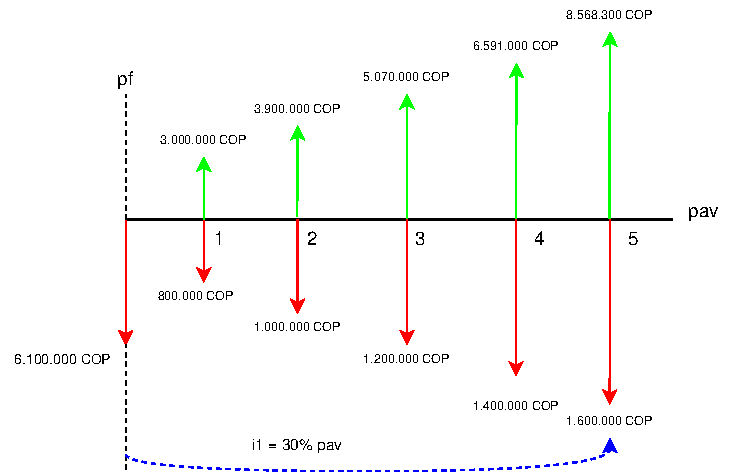
\includegraphics[trim=-5 -5 -5 -5 , scale=0.4]{9_Capitulo/ejemplos/7/Capitulo9Ejercicio7.pdf}}  \\ \hline
		%%%%%%%%%%%%% FIN INSERCION DE IMAGEN
		%%%%%FIN FLUJO DE CAJA



		%%%%% INICIO DECLARACION FORMULAS
		%%%%%%%%%%% INICIO TITULO
		\rowcolor[HTML]{FFB183}
		\multicolumn{3}{|c|}{\cellcolor[HTML]{FFB183}\textbf{4. Declaración de fórmulas}}    \\ \hline
		%%%%%%%%%%% FIN TITULO
		%%%%%%%%%%% INICIO MATEMATICAS
		\multicolumn{3}{|c|}{$FLUJO\_DE\_CAJA\_LIBRE\_DEL\_PROYECTO= UTILIDADES\_ANTES\_DE\_IMPUESTOS$}\\
		\multicolumn{3}{|c|}{$+ INTERESES+ DEPRECIACIONES + AMORTIZACIONES - IMPUESTOS - INVERSIONES$}\\
		\multicolumn{3}{|c|}{$IMPUESTOS=(UTILIDADES\_ANTES\_DE\_IMPUESTOS+INTERESES)*TASA\_IMPOSITIVA$} \\ \hline
		%%%%%%%%%% FIN MATEMATICAS
		%%%%%% INICIO DESARROLLO MATEMATICO
		\rowcolor[HTML]{FFB183}
		%%%%%%%%%%INICIO TITULO
		\multicolumn{3}{|c|}{\cellcolor[HTML]{FFB183}\textbf{5. Desarrollo matemático}}       \\ \hline
		%%%%%%%%%% FIN TITULO
		%%%%%%%%%% INICIO MATEMATICAS
		\multicolumn{3}{|c|}{}\\ 
		\multicolumn{3}{|c|}{\textbf{1. Usando el flujo de caja para el accionista (FCLA):}}\\ 
        		\multicolumn{3}{|c|}{
		\resizebox{\textwidth}{!}{%
        			\begin{tabular}{|c |c |c |c |c |}                                                             \hline
                            	AÑO                         & 0            & 1            & 2            & 3            \\ \hline
                            	INGRESOS                    & --           & 7.000.000 COP  & 7.000.000 COP  &  7.000.000 COP \\ \hline
                            	EGRESOS                     & --           & 1.000.000 COP  & 1.000.000 COP  & 1.000.000 COP  \\\hline
                            	DEPRECIACIÓN                & --           & 2.666.667 COP  & 2.666.667 COP & 2.666.666 COP  \\ \hline
                            	UTILIDAD BRUTA              & --           &  3.333.333 COP & 3.333.333 COP  &  3.333.334 COP \\\hline
                            	GASTOS OPERACIONALES        & --           & 0 COP          & 0 COP          & 0 COP          \\\hline
                            	UTILIDAD OPERACIONAL        & --           &  3.333.333 COP & 3.333.333 COP  &  3.333.334 COP \\\hline
                            	GASTOS FINANCIEROS          & --           & 600.000 COP   & 435.162 COP    &  237.363 COP   \\\hline
                            	UTILIDAD ANTES DE IMPUESTAS & --           &  2.733.333 COP & 2.898.168 COP  & 3.095.971 COP  \\\hline
                            	INVERSIONES                 & 5.000.000 COP  & --           & --           & \ --         \\\hline
                            	AMORTIZACIÓN                & --           &  824.176 COP   & 989.011 COP    &  1.186.813 COP \\\hline
                            	DEPRECIACIONES              & --           &  2.666.667 COP & 2.666.667 COP  &  2.666.666 COP \\\hline
                            	FNC PARA INVERSIONISTAS     & -5.000.000 COP &  3.619.157 COP & 3.561.465 COP  &  3.492.234 COP \\\hline
                            	TIO                         & 40\%         & VA           &  674.867 COP       &           \\\hline
                        \end{tabular}}
		}\\ 
		\multicolumn{3}{|c|}{}\\
		\multicolumn{3}{|c|}{\textbf{2. Usando el flujo de caja libre del proyecto (FCLP):}}\\
        		\multicolumn{3}{|c|}{
		\resizebox{\textwidth}{!}{%
        			\begin{tabular}{ |c | c| c| c| c|}
                    		\hline
                    		AÑO                         & 0  & 1            & 2           & 3           \\\hline
                    		UTILIDAD ANTES DE IMPUESTAS & -- &  2.733.333  COP & 2.898.168  COP & 3.095.971 COP \\\hline
                    		+ INTERESES (20\%)          & -- & 600.000 COP    & 435.165 COP   & 237.363 COP   \\  \hline
                    		IMPUESTOS                   & -- & 1.166.667 COP  & 1.166.667 COP & 1.166.667 COP \\  \hline
                    	\end{tabular}}
		}\\
		\multicolumn{3}{|c|}{}\\ 
		\multicolumn{3}{|c|}{\textbf{FLUJO DE CAJA LIBRE PROYECTO:}}\\
        		\multicolumn{3}{|c|}{
		\resizebox{\textwidth}{!}{%
        			\begin{tabular}{ |c | c| c| c| c|}
                    		\hline
                    		AÑO                         & 0            & 1            & 2           & 3                \\\hline
                    		UTILIDAD ANTES DE IMPUESTAS & --           & 2.733.333 COP & 2.898.168 COP & 3.095.971 COP      \\\hline
                    		INTERESES                   & --           & 600.000 COP    & 435.165 COP   & 237.363 COP        \\  \hline
                    		IMPUESTOS                   & --           & 1.166.667 COP  & 1.166.667 COP & 1.166.667 COP      \\  \hline
                    		DEPRECIACIONES              & --           &  2.666.667 COP & 2.666.667 COP & 2.666.666 COP      \\\hline
                    		INVERSIONES                 & -8.000.000 COP &  4.833.333 COP & 4.833.333 COP & 4.833.333 COP      \\\hline
                    		F.C LIBRE DEL PROYECTO      & -320.214 COP  & TIO =  40\%  & TIO =  40\% & VAN = -320.214 COP \\\hline
                    	\end{tabular}}
		}\\ 
		\multicolumn{3}{|c|}{}\\ \hline

		%%%%%%%%%% FIN MATEMATICAS
		%%%%%% FIN DESARROLLO MATEMATICO
		%%%%%% INICIO RESPUESTA
		\rowcolor[HTML]{FFB183}
		%%%%%%%%%%INICIO TITULO
		\multicolumn{3}{|c|}{\cellcolor[HTML]{FFB183}\textbf{6. Respuesta}}   \\ \hline
		%%%%%%%%%% FIN TITULO
		%%%%%%%%%% INICIO RESPUESTA MATEMATICA
		\multicolumn{3}{|c|}{En conclusión el proyecto no es bueno, debido a que si bien el flujo de caja del inversionista}  \\ 
		\multicolumn{3}{|c|}{es de 674.867 COP, el del accionista marca perdidas con un valor de 320.214 COP.}\\
		\multicolumn{3}{|c|}{Por lo tanto, no satisface a las dos partes.}\\ \hline
		%%%%%%%%%% FIN MATEMATICAS
		%%%%%% FIN RESPUESTA
	\end{longtable}
	%Se crean dos lineas en blanco para que no quede el siguiente texto tan pegado
	%\newline \newline %USARLO SI CREES QUE ES NECESARIO
\end{center}
%%%%%%%%%%%%%%%%%%%%%%%%%%FIN EJERCICIO 1 %%%%%%%%%%%%%%%%%%%%%%%%%%%
